
\documentclass{article}
\usepackage{graphicx}
\usepackage{minted}
\usepackage{parskip}
\usepackage{hyperref}

\definecolor{bg}{rgb}{0.95, 0.95, 0.95}
\begin{document}
\section*{Scalars, Vectors and Matrices}

We referred loosely to a set of numbers enclosed in square brackets
as a `series' in the previous session. Matlab calls these \emph{vectors}. 
Here are a few ways of generating vectors in Matlab:

\begin{minted}[bgcolor=bg]{octave}
    
    >> a = [3.5, 7.4, 3.3, 9.01]; % Manually entering values
    >> b = 1:0.5:10;              % For a specified spacing
    >> c = linspace(0, 1, 100);   % 100 evenly-spaced values 
                                  % from 0 to 1
\end{minted}

You can do a bunch of things with vectors, for instance:

\begin{minted}[bgcolor=bg]{octave}
    
    >> a = [3.5, 7.4, 3.3, 9.01];
    >> max(a)
    >> min(a)
    >> mean(a)
    >> length(a)

\end{minted}

But vectors are only a part of the more general class of \textbf{Matrices}.
Generate a matrix:

\begin{minted}[bgcolor=bg]{octave}

    >> A = [1, 2; 3, 4] % Separate rows with semicolons
    >> M = zeros(3, 5)  % Matrix of zeros, 3 rows, 5 columns
    >> N = ones(5)      % A `square' 5-by-5 matrix of ones
    >> size(M)
    >> M'               % `Transpose' the matrix

\end{minted}

\subsection*{Accessing elements of vectors and matrices}

\begin{minted}[bgcolor=bg]{octave}

    >> v = range(1, 10)     % Generate a vector
    >> M = [1:4; 5:8; 9:11] % Generate a matrix from three 
                            % vectors
    
    >> v(4)                 % The 4th element of `v'
    >> M(2, 3)              % The element of `M' sitting in
                            % the 2nd row and 3rd column

    >> v(2:5)               % Elements 2 through 5 of `v'
    >> M(2, 1:3)            % Row 2, columns 1 through 3
    >> v(3:end)             % All elements starting from the 3rd
    >> M(2:end, 2:end)      % All the elements sitting in columns
                            % 2-through-end of rows 2-through-end
\end{minted}

\pagebreak

This may all be a bit overwhelming, but we cannot emphasize enough:

\fbox{
  \parbox{\textwidth}{
   Learning to \textbf{generate}, \textbf{manipulate} and 
   \textbf{operate on} vectors and
   matrices is \underline{the key} to writing good
   Matlab code!
  }
}
\section*{Exercise}

Okay, let's jump right in to an interesting application of
matrices - manipulating images!

\begin{figure}[h]
\begin{center}
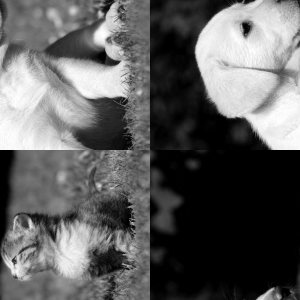
\includegraphics[height=150pt]{figures/faceoff.png}
\end{center}
\end{figure}

A grayscale image is just a matrix of numbers. Each `pixel' has
a certain \emph{intensity}. An intensity of 0 corresponds to black,
and an intensity of 255 corresponds to white. All numbers in between
correspond to increasingly lighter shades of gray. If you're curious,
color images work the same way, except we need three matrices, each
one representing the intensities of Red, Green and Blue.

Load the image on to Matlab:

\begin{minted}[bgcolor=bg]{octave}
    >> M = imread('faceoff.png');
    >> size(M) % Gives the number of pixels in each direction 
               % (`dimensions')
\end{minted}

Of course, you don't need Matlab to check the image dimensions.

The objective of this exercise should be obvious: fix the image, given that
each `quarter' of the image is a 150 x 150 sub-image.

\end{document}